\documentclass[conference]{IEEEtran}

% *** GRAPHICS RELATED PACKAGES ***
%
\ifCLASSINFOpdf
  % \usepackage[pdftex]{graphicx}
  % declare the path(s) where your graphic files are
  % \graphicspath{{../pdf/}{../jpeg/}}
  % and their extensions so you won't have to specify these with
  % every instance of \includegraphics
  % \DeclareGraphicsExtensions{.pdf,.jpeg,.png}
\else
  % or other class option (dvipsone, dvipdf, if not using dvips). graphicx
  % will default to the driver specified in the system graphics.cfg if no
  % driver is specified.
  % \usepackage[dvips]{graphicx}
  % declare the path(s) where your graphic files are
  % \graphicspath{{../eps/}}
  % and their extensions so you won't have to specify these with
  % every instance of \includegraphics
  % \DeclareGraphicsExtensions{.eps}
\fi
% graphicx was written by David Carlisle and Sebastian Rahtz. It is
% required if you want graphics, photos, etc. graphicx.sty is already
% installed on most LaTeX systems. The latest version and documentation
% can be obtained at: 
% http://www.ctan.org/pkg/graphicx
% Another good source of documentation is "Using Imported Graphics in
% LaTeX2e" by Keith Reckdahl which can be found at:
% http://www.ctan.org/pkg/epslatex
%
% latex, and pdflatex in dvi mode, support graphics in encapsulated
% postscript (.eps) format. pdflatex in pdf mode supports graphics
% in .pdf, .jpeg, .png and .mps (metapost) formats. Users should ensure
% that all non-photo figures use a vector format (.eps, .pdf, .mps) and
% not a bitmapped formats (.jpeg, .png). The IEEE frowns on bitmapped formats
% which can result in "jaggedy"/blurry rendering of lines and letters as
% well as large increases in file sizes.
%
% You can find documentation about the pdfTeX application at:
% http://www.tug.org/applications/pdftex
\usepackage{graphicx}
\graphicspath{{images/}}
\usepackage{array}
\usepackage{caption}
\usepackage{placeins}
\usepackage{amsmath}
\usepackage{amsfonts}
\newcolumntype{P}[1]{>{\centering\arraybackslash}p{#1}}

\hyphenation{op-tical net-works semi-conduc-tor}


\begin{document}
\title{Cardiovascular Health Prediction with Bayesian Network}


% author names and affiliations
% use a multiple column layout for up to three different
% affiliations
\author{\IEEEauthorblockN{Phillip Osial, Kalle Kauranen}
\IEEEauthorblockA{Department of Computer Science\\
Lakehead University\\
Thunder Bay, Ontario, Canada\\
pgosial@lakeheadu.ca, kakauran@lakeheadu.ca}}

\maketitle

\begin{abstract}
In Canadian society, the ubiquity of cardiovascular disease has led to it becoming the second leading cause of death for Canadians. In this paper, we examine the process of creating a clinical decision support system using a Bayesian Network to model and identify the risk factors associated with a diagnosis of cardiovascular disease. With this research, we hope to increase the preventative techniques available to Canadian citizens and provide a better quality of life for all.
\end{abstract}

\IEEEpeerreviewmaketitle

\section{Introduction}
Cardiovascular disease (CVD) is part of a category of diseases involving the heart and blood vessels that is now the \textit{second leading} cause of death in Canada \cite{StatsCan}. As a result of its increasing prevalence, large amounts of research is being conducted to try and bring down the instances of death and increase the health of Canadians from coast-to-coast. To accomplish our analysis, we will create a \textit{Bayesian Network} to model our clinical decision making process (CDMS). Afterwards, we evaluate our CDMS using a receiver operating characteristic (ROC) curve and determine the area under the curve (AUC).  
\subsection{Defining Datasets}

\section{Research Motivation}
Nowadays there is a large focus in research in what is called Big Data Analytics (BDA). BDA is the process of analyzing large amounts of data to find hidden patterns and meaning within. Examples of where BDA is making large improvements are the pharmaceutical industry where BDA is allowing researchers to focus on the medications that will be most likely to succeed and in the cases of disease and viral outbreaks where BDA is mapping out the genetic components that are able to stop the diseases from spreading. Our end goal for this research also focuses on the health industry but looks at creating a process for predicting cardiovascular disease in order to hopefully prevent it in the overall Canadian population. An example applicable to our domain follows:
\\
\indent A person goes for a checkup at their family physician. At the checkup they are given a survey to fill out and are run through the usual set of tests. The results from the survey and the tests are then run through the clinical decision making process to determine problem areas of the individual that put them at risk for CVD. Using the results, the individual can take that knowledge and change his lifestyle habits to decrease his likelihood of CVD.
\\
\indent This one example shows a possible usage for the research that will be gained here.

\section{Related Works}
Research in cardiovascular health has steadily increased over the years as it has become more common in the health care fields. Advancements and usage of big data analytics has improved the methods and variety of research that can be conducted on the existing datasets. 
Looking at what was proposed by Sultana et al \cite{7873142}, they analyzed several different heart disease prediction techniques. Through their research they found that Bayes Net and SMO classifiers performed best among their initial five classifiers: Bayes Net, SMO, KStar, MLP and J48. To come up with this conclusion the five classifiers were tested against two sets of data, the UCI standard heart disease dataset as well as collected patient data from Bangladesh. Using the accuracy calculated from the True Positive Rate (TPR) and the False Positive Rate (FPR) as well as the AUC from the ROC curve, Bays Net and SMO were found to be the best of the classifiers tested.
   Raihan et al \cite{7860213} proposes a smartphone application heart disease prediction system with data mining techniques. Their proposed system in theory is able to predict Ischemic Heart Disease from a smartphone interface. They suggested that main tools that have a mandatory input of lipid values make them underutilized by the population at large. While such tools are valuable they set out to make a system that is more user friendly to a non medical professional. 
   Rosli et al \cite{7808353} proposes another mobile detection system for heart disease but this time looking for early warning signs of fatal heart disease. Their system also uses an Arduino micro-controller to measure the heart rate of the individual. Their system uses photoplethysmography technique and utilizes a GSM shield module to act as an SMS interface. In a survey to test the effectiveness of their system, 100\% of respondents agreed that their system is relevant for the industry.
\section{Data Description}
Our research focused on two datasets. We first examined the standard statlog heart disease dataset from UCI machine learning repository \cite{StatlogHeart}.  The data attributes can be seen in Table \ref{table_statlogheart}.  The data contains multivariate characteristics consisting of both numerical and categorical data types.
This dataset also features no missing values, contains 270 rows with 14 attributes, and its primary purpose is to be used for prediction of heart disease by using the first 13 attributes as predictors of the 14\textsuperscript{th} attribute.
Our second dataset consisted of a subset of the Canadian Heart Health Survey Dataverse \cite{HealthSurvey}. The dataset produced in 1997 contains the data from ten Heart Health Surveys conducted between 1986 and 1992 in Canada. The dataset is also much more extensive than our starting set containing 23129 rows and 266 attributes of which we only used a smaller subset to produce our clinical decision support (CDS) model.
Our smaller subset consisted of examining only 37 attributes and a snapshot of some of the attributes examined can be seen in Table \ref{table_heartsurvey}.

\begin{table}[!ht]
\begin{center} 
\caption{Statlog Heart Dataset \cite{StatlogHeart}}
\begin{tabular}{ |P{0.3cm}|P{4.0cm}|P{1.4cm}|P{1.4cm}|}
\hline 
\#	&	Attribute										& Abbreviation & Data Type\\
\hline
1	&	Age											& age & Numeric\\
 \hline
2 	&	Sex											& sex & Categorical\\
\hline
3	&	Chest Pain Type (4 vals)								& cpt & Categorical\\
\hline
4 	&	Resting Blood Pressure								& rbp & Numeric\\
\hline
5 	&	Serum Cholesterol in mg/dl								& sc & Numeric\\
 \hline
6 	&	Fasting Blood Sugar $>$ 120 mg/dl 						& fbs & Categorical\\
 \hline
7 	&	Resting Electrocardiographic Results (Values 0,1,2) 				& recg & Categorical\\
 \hline
8 	&	Maximum Heart Rate Achieved 							& mhr & Numeric\\
 \hline
9 	&	Exercise Induced Angina 								& eia & Categorical\\
 \hline
10 	&	Oldpeak = ST Depression Induced by Exercise Relative to Rest 		& op & Numeric\\
 \hline
 11 	&	The Slope of the Peak Exercise ST Segment 					& sop & Categorical\\
 \hline
 12 	&	Number of Major Vessels (0-3) Colored by Flourosopy 			& nmv & Numeric\\
 \hline
 13 	&	Thal: 3 = Normal; 6 = Fixed Defect; 7 = Reversible Defect 			& thal & Categorical\\
 \hline
 14 	&	Heart Disease Absent (1) or Present (2) 					& hdap & Categorical\\
 \hline
\end{tabular}
\label{table_statlogheart}
\end{center}
\end{table}

\begin{table}[!ht]
\begin{center} 
\caption{Heart Survey Dataset \cite{HealthSurvey}}
\begin{tabular}{ |P{0.3cm}|P{4.0cm}|P{1.4cm}|}
\hline
\#	&	Attribute										& Abbreviation\\
\hline
1	&	Age Grouped in 10 Year Segments					& gpage2\\
 \hline
2 	&	Sex											& sex\\
\hline
3	&	BMI Categories								& bmicat\\
\hline
\multicolumn{1}{|c|}{\vdots} 	&	\multicolumn{1}{c|}{\vdots} 	& \multicolumn{1}{c|}{\vdots}\\
\hline
35 	&	Other Heart Disease								& othhd\\
 \hline
36	&	Ever Had a Heart Attack?							& everha\\
 \hline
37 	&	Ever Had a Stroke?								& everstr\\
 \hline
\end{tabular}
\label{table_heartsurvey}
\end{center}
\end{table}

\section{Methodology} 
For the first dataset, Table \ref{table_statlogheart}, we simplified our analysis by only using data that was already categorical since categorizing the numerical data could be considered subjective.
The main attributes we considered were sex, thal, hdap, cpt, recg, eia, sop, and fbs.
First, we created an undirected Bayesian Network as seen in Fig. \ref{fig_statloghealth_undirected}. 
We quickly realized that this would of no use to us because we cannot see the direct dependencies between attributes.
This led us to creating a directed Bayesian Network as seen in Fig. \ref{fig_statloghealth}.
The Bayesian Network we created uses the \textit{Hill Climbing} approach to ensure in a completely directed network.
From this directed Bayesian Network, Fig. \ref{fig_statloghealth}, we are able to see how certain attributes depend upon each other.
Since the first dataset, Table \ref{table_statlogheart}, was too small, we looked at another dataset and took a subset of the data, Table \ref{table_heartsurvey}, to perform further analysis.
This dataset comprised mainly of categorical data so it allowed us to have a large amount of data even after omitting numerical data.

\section{Results and Discussion}
In this section, we discuss the results of our constructed Bayesian Networks as well as our ROC curve.
\subsection*{Table \ref{table_statlogheart}: Undirected Bayesian Network}
Using the undirected Bayesian Network as seen in Fig. \ref{fig_statloghealth_undirected}, we were able to run tests against this model and determine the highest and lowest factors for heart disease.
\begin{figure}[!ht]
\centering
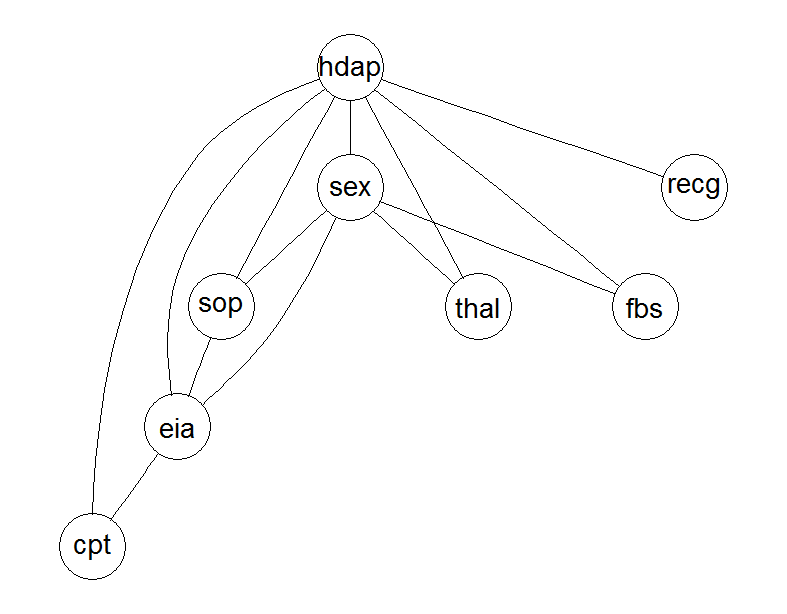
\includegraphics[width=\columnwidth]{bn_statloghealth_undirected}
\caption{Undirected Bayesian Network}
\label{fig_statloghealth_undirected}
\end{figure}

We discovered that the highest probability for heart disease followed conditions as seen in Table \ref{table_hdap_highest}.

\begin{table}[!ht]
\begin{center} 
\caption{Highest Heart Disease Probability (99.84\%)}
\begin{tabular}{|P{1.4cm}|P{4.5cm}|}
\hline 
Abbreviation & Value \\
\hline
sex & Female\\
\hline
cpt & Asymptomatic\\
\hline
fbs & Fasting Blood Sugar $>$ 120 mg/dl\\
\hline
recg & Showing Probable/Definite Left Ventricular Hypertrophy by Estes’ Criteria\\
\hline
eia & Yes\\
\hline
sop & Flat\\
\hline
thal & Reversible defect\\
\hline
\end{tabular}
\label{table_hdap_highest}
\end{center}
\end{table}

We were also able to discover that the lowest probability for heart disease followed conditions as seen in Table \ref{table_hdap_lowest}.

\begin{table}[!ht]
\begin{center} 
\caption{Lowest Heart Disease Probability (0.063\%)}
\begin{tabular}{|P{1.4cm}|P{5.0cm}|}
\hline 
Abbreviation & Value \\
\hline
sex & Female\\
\hline
cpt & Typical Angina\\
\hline
fbs & Fasting Blood Sugar $<$ 120 mg/dl\\ 
\hline
recg &  Normal\\
\hline
eia & Yes\\
\hline
sop & Upsloping\\
\hline
thal & Normal\\
\hline
\end{tabular}
\label{table_hdap_lowest}
\end{center}
\end{table}


For our second dataset we created the network seen in Fig. \ref{fig_heartsurvey}. This Baysian network contains 37 nodes and 75 arcs with all of them being of the directed variety. The markov blanket size which indicates the number parents, children and parents of the children of the node was 5.19. 

\begin{figure}[!ht]
\centering
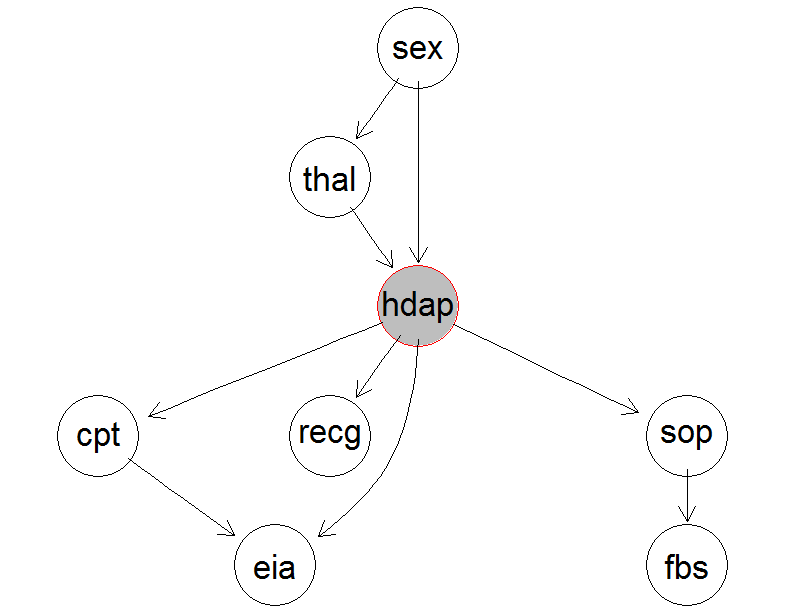
\includegraphics[width=\columnwidth]{bn_statloghealth}
\caption{Directed Bayesian Network}
\label{fig_statloghealth}
\end{figure}


\begin{figure*}[!ht]
\centering
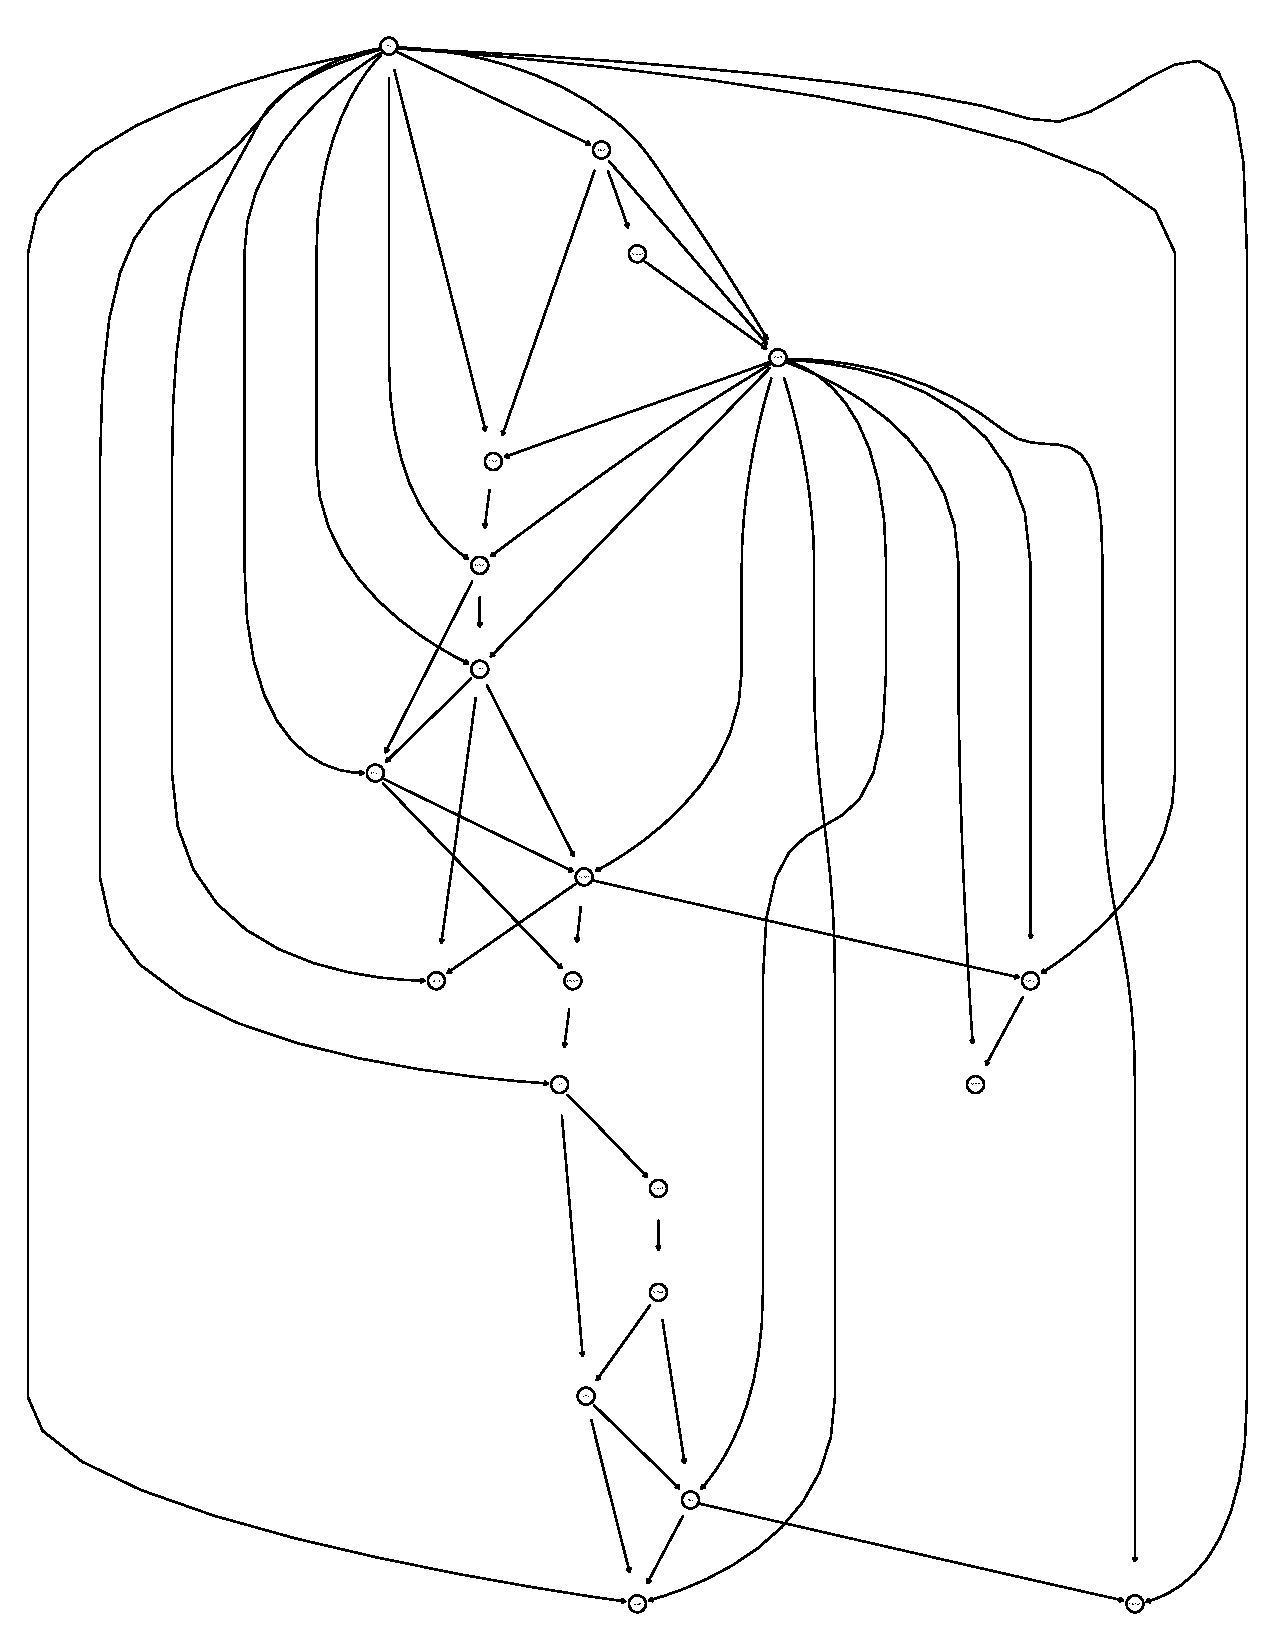
\includegraphics[width=\textwidth]{bn_heartsurvey.pdf}
\caption{Directed Bayesian Network Using Heart Survey}
\label{fig_heartsurvey}
\end{figure*}

\section{Conclusion and Future Work}

\bibliography{mybib}{}
\bibliographystyle{plain}




% End of document
\end{document}


